\documentclass[main.tex]{subfiles}

\begin{document}
\section{Overview}
A large number of charged cosmic ray events are included among the triggering events despite the three-level trigger. Most current generation experiments use analysis techniques based on Hillas parameters \cite{Hillas:1985}, using the second moments of the distribution of pixel signal amplitudes, which for VERITAS, yield an angular resolution of $\sim <0.1^\circ$ at 1 TeV. However, significantly more information can be extracted from the recorded data using a template library containing expected shower images for a given set of shower parameters. This template library can then be compared to the recorded images for any given event and the best-fit shower parameters can be determined resulting in improved resolution in direction and energy reconstruction. This section provides a brief overview of the Monte-Carlo simulations used to generate these templates for VERITAS.

\section{Shower Generation}
This section describes the prediction of the expected Cherenkov light distribution in the camera focal plane for a given set of primary particle parameters. The production of mean shower images is divided into two steps: the generation of large Monte Carlo datasets of air showers and the simulation of the detector response. The electromagnetic air showers in the atmosphere are simulated with the CORSIKA (COsmic Ray SImulations for KAscade) program and simulations are performed over a range of parameters like energy, zenith angle and impact distance. 

In the simulation, which contains the shower generation from \ref{Gamma-ray-EAS}, when a charged particle exceeds $v>c/n$, Cherenkov photons are generated. The number of photons emitted is calculated for a given extent of the path and the propagation directions are randomly selected from the surface of a Cherenkov cone (i.e. $\theta_c = \cos^{-1}\beta/n$). Each photon is then tracked through the atmosphere until it reaches the altitude of the observatory. CORSIKA does not track whether the photon hits a telescope reflector, but instead defines a volume around each telescope in order to filter photons to store. Photons whose trajectory does not intersect this volume are not stored.

With the instrument pointing at the shower source, each of the telescope cameras lies on a plane perpendicular to the shower axis, making the shower projection plane and the camera planes parallel. The CORSIKA simulation output contains the photon distribution at the telescope altitude, and the arrival direction of each photon. For each event, the Cherenkov photons falling onto the mirror elements are tracked by their arrival times, initial direction, and wavelength. The detector response is modeled using the atmospheric density profile, optical absorption and some of the detector characteristics such as its light-collecting area, and phototube quantum efficiency. It also accounts for the physical structure of the telescopes such as occultation by the quadripod arms and the camera box. The images are produced for the VERITAS telescopes which use a Davies-Cotton design and cameras with 499 pixels, each pixel having a field of view (FOV) of 0.15$^\circ$ in diameter.

The shower images are generated for a range of first-interaction depths, energies, wobble offsets and impact distances. A multidimensional interpolation algorithm is used to interpolate between the templates, allowing production of an image template for any shower parameters within the parameter ranges. An additional parameter included here is the effect of the geomagnetic field on the electromagnetic showers \cite{Vincent:2015bnj}.
% 3. Likelihood Reconstruction & Performance
Once the full set of templates has been created, they can be compared with the observed images by performing a global fit to the telescope image data using a model for the expected pixel amplitudes. Shower parameters are determined by maximizing an array likelihood function, as outlined in \cite{deNaurois}.

\section{The VEGAS Analysis Package}
The VERITAS observation and simulation data contain the PMT pulses, pointing direction, time and time gradient (which are extracted from the PMT pulses), and other trigger and operational conditions. To produce a sky map, these data files are piped through a series of functions to extract, among other things, energy and direction information. At VERITAS there are two standard analysis packages for this process (\vegas  and \ed), both based in ROOT/C++, with a similar set of functions. While the analysis methods in this work can be and are applied in both analysis packages, the analysis in this work was performed using the \vegas package.
\vegas consists of 6 distinct processes, initially written as 6 distinct modules, as follows:
\begin{itemize}
\item Stage 1: Calibration Calculation -- This stage calculates the hardware dependent parameters of the VERITAS data and collects relevant information at each trigger level (pixel, telescope, and array) to determine a set of calibration parameters. The following stages can then use these parameters in conjunction with the data to remove any hardware dependence.
\item Stage 2: Calibration Application -- This stage calculates calibrated charge information for PMT traces using information on pedestals, relative gains, and relative channel timing. In more recent iterations, the analysis module for stage 2 also performs the functions previously performed in stage 3. 
\item Stage 3: Image Parameterization -- This stage removes noisy pixels using stage 1 \& 2 information and calculates the image parameters (described in \ref{shower-img-params}). This stage treats each telescope independently and so image parameters are calculated for each telescope image.
\item \textbf{Stage 4: Shower Reconstruction} -- This is the most important stage for the purposes of this work. This stage performs an array-level reconstruction of the shower, using individual telescope information to calculate \textbf{shower direction} (the original arrival direction of the candidate photon), event energy, depth of the shower maximum, and core location.
\item Stage 5: Event Selection -- This stage is designed to apply cuts to events based on the output of the previous stages to better distinguish hadronic showers from gamma-ray showers, as well as enforce any other restrictions on telescope-image or stereoscopic parameters.
\item Stage 6: Results Extraction -- This stage calculates and displays the final results of the desired analysis -- single telescope analysis, stereoscopic analysis, spectral analysis or temporal flux analysis.
\end{itemize}
The focus of this work will be on the direction reconstruction part of stage 4.

\section{Direction Reconstruction}
\begin{figure}[htbp]
  \centering
  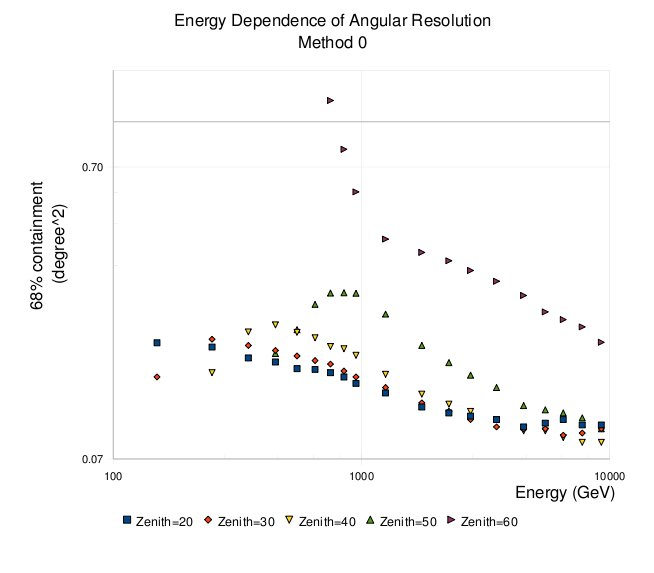
\includegraphics[width=.6\linewidth]{images/Method0_res}
  \caption[Angular resolution of Method0.]{Angular resolution of Method0 direction reconstruction as a function of energy scale and zenith angle. From \cite{veritas_web}.}
  \label{fig:disp_res}
\end{figure}
The standard method (henceforth method0) of shower direction reconstruction is based on the intersections of the major axes of Hillas ellipses (see Fig. \ref{fig:hillas_ellipse}). This method carries a lot of stereoscopic information and is in general very powerful. However, for large zenith angles (LZA), one expects shower images (and therefore Hillas ellipses) in the camera plane to be from the same region in the lightpool (see Fig. \ref{fig:LZA_lightpool}) and close to parallel, so that small uncertainties in major axis determination result in large uncertainties in the fiducial location of the reconstructed gamma ray in the camera plane (the ``shower location''). As shown in Fig. \ref{fig:disp_res}, for lower energies and at larger zenith angles, there is a substantial degradation in angular resolution.

\begin{figure}[htbp]
  \centering
  \subfigure[The light pool for Cherenkov showers at small zenith angle versus at large zenith angle. Picture taken from \cite{hess_web}.]{
  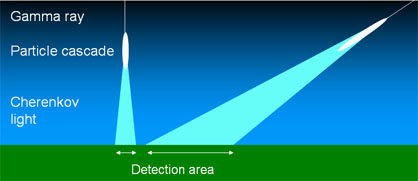
\includegraphics[width=.8\linewidth]{images/LZA_lightpool}
}
\subfigure[The Hillas ellipses resulting from two telescopes at LZA.]{
  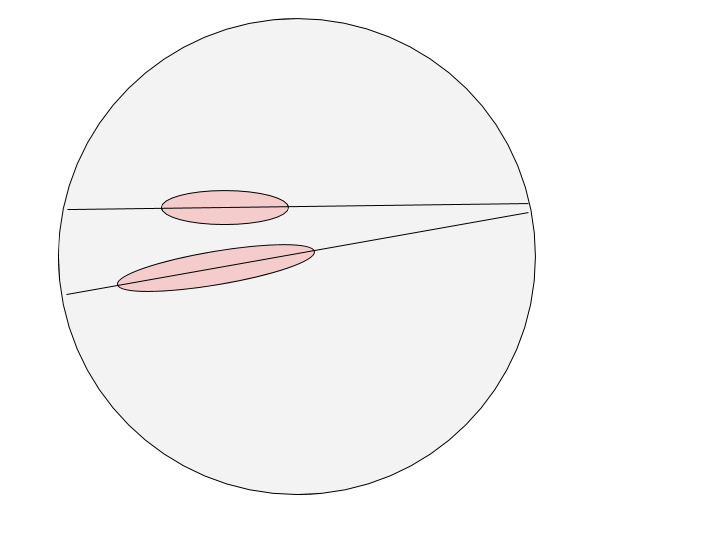
\includegraphics[width=.60\linewidth]{images/LZA_stereo_ellipse}
}
  \caption[Stereoscopic reconstruction at LZA.]{The stereoscopic method is less effective at large zenith angles due to the lightpool from these events being much larger than the coverage of the telescopes. This results in the telescopes being in the same region of the light pool and therefore nearly parallel Hillas ellipses. In such cases, the stereoscopic method of reconstruction will have a large uncertainty in the point of intersection of these two axis, which corresponds to a large uncertainty in the reconstructed direction.}
  \label{fig:LZA_lightpool}
\end{figure}


\subsection{The \disp Method}
To compensate for this loss of predictive power, the \disp \textit{method}, calculates the \disp parameter (quasi-analytically, using lookup tables and interpolating, or using \textbf{boosted decision trees}) for each individual telescope image to determine two potential locations for the arrival direction -- along the major axis on either side of the weighted centroid of the image (see Fig. \ref{fig:hillas_ellipse}). This parameter is the (angular) vector displacement between the weighted centroid of the shower image and the estimated arrival direction of the initiating photon. In addition, the method also determines the two-dimensional uncertainty on this parameter which is expressed in terms of the radial ({\it DispError}) and angular ({\it MAError}) uncertainties. Together, these three parameters fully specify the direction of the initiating photon and the uncertainty on it, up to the head-tail ambiguity.

The method then compares this pair of coordinates (one at the head, and one at the tail) for each pair of telescopes in the event reconstruction to find the pair of coordinates, one from either telescope, that are closest to each other (see Fig \ref{fig:head_tail} for visual explanation). The weighted mean of this pair of coordinates is taken as the reconstructed shower direction, with the weights given by {\it DispError} and {\it MAError}. The RMS distance of the two closest points (the points in the red circle in Fig. \ref{fig:head_tail_full}) is taken to be the uncertainty on this position.
\begin{figure}[htbp]
  \centering
\subfigure[First pair of telescopes in reconstruction, with the pair of closest coordinates.]{
  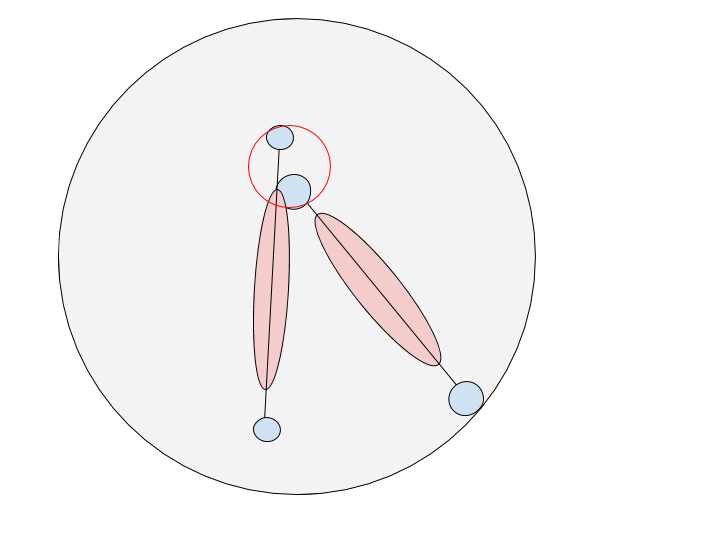
\includegraphics[width=.31\linewidth]{images/head_tail_1}
}
\subfigure[Second pair of telescopes in reconstruction, with the pair of closest coordinates.]{
  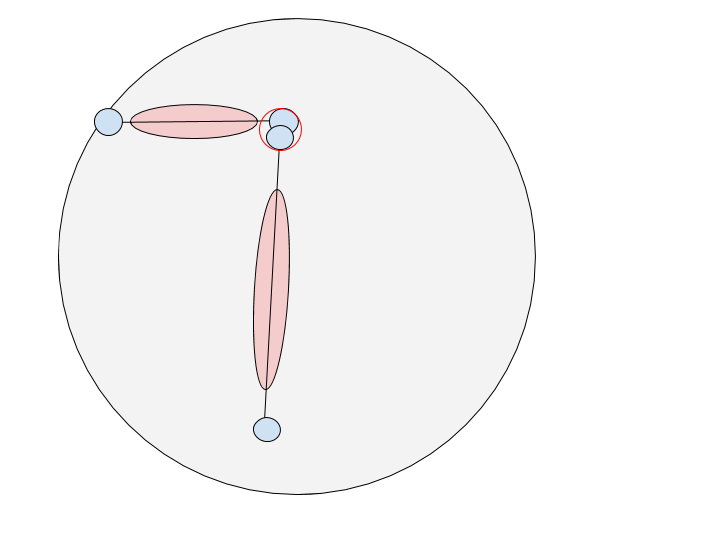
\includegraphics[width=.31\linewidth]{images/head_tail_2}
}
\subfigure[Third pair of telescopes in reconstruction, with the pair of closest coordinates.]{
  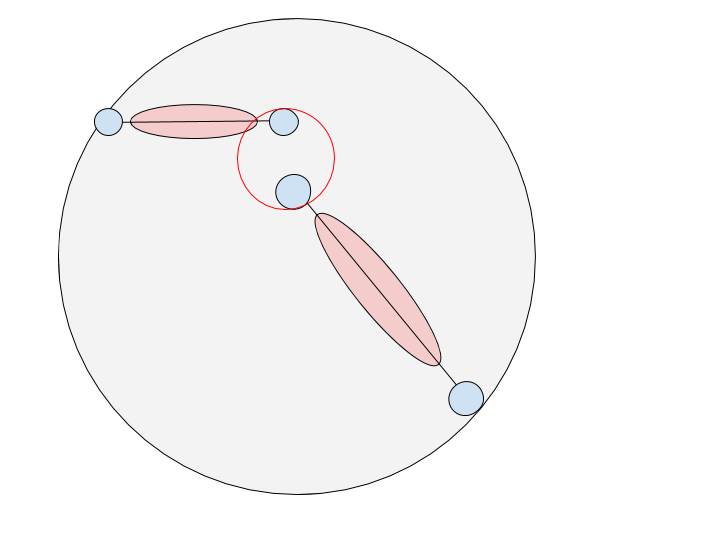
\includegraphics[width=.31\linewidth]{images/head_tail_3}
}
\subfigure[All telescopes in reconstruction, with the pair of closest coordinates from \textit{all} pairs of telescopes.]{
  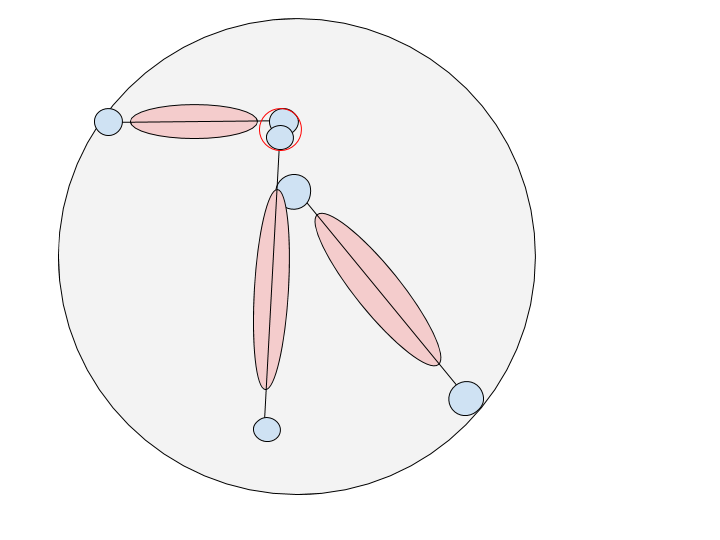
\includegraphics[width=.6\linewidth]{images/head_tail_full}
  \label{fig:head_tail_full}
}
  \caption[Combining multiple telescopes in \disp reconstruction.]{Iterating through the unique pairs of telescopes, the closest coordinate pair is chosen, and the mean of those coordinates is taken as the direction of the initiating particle.}
  \label{fig:head_tail}
\end{figure}

While using a quasi-analytic lookup table already provides substantial improvements on the LZA performance of the direction reconstruction, using boosted decision trees (BDTs) provides significantly better resolution comparable to (and in some regimes better than) that from the geometric reconstruction in the medium zenith angle range ($40^\circ-50^\circ$).

\section{Boosted Decision Trees}
Decision trees use a predictive model, which maps parameters for an event to the value of the \disp parameter for the event. For example, Fig. \ref{fig:BDT_flowchart} shows a decision tree that uses observed quantities to determine the temperature outside. The tree starts at the ``root node'', which is the first test or question posed on the input data. The answer to this test determines the ``branch'' of the tree that is followed (in Fig. \ref{fig:BDT_flowchart}, Sunny or Overcast). Branches lead to ``nodes,'' which can either terminate (``leaf-nodes''), providing an answer, or pose a question and branch out again (``non-leaf nodes'') as demonstrated in Fig. \ref{fig:BDT_flowchart}.

The questions asked at each point are determined from a predictive model which may be based on analytic calculations (as in this example), or on Monte Carlo simulations (as in the case of this work). A basic algorithm for boosted decision tree (BDT) learning takes an input sample of data, generates a decision tree, uses a boosting algorithm to better discriminate mis-modeled inputs, and runs tests to provide some measures of its own performance. BDTs are especially robust for variables with non-linear correlations and have a fast application to data, relative to some other algorithms. This section contains a brief description of these individual steps.
\begin{figure}[htbp]
  \centering
  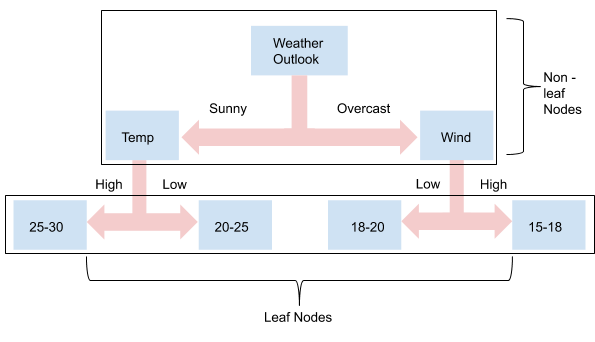
\includegraphics[width=.9\linewidth]{BDT_flowchart}
  \caption[An example of a BDT]{An example of a BDT to determine the temperature using observables. Each test or question is represented by a ``node,'' which creates two or more ``branches'' of the tree. Each of these branches represent a particular answer (or set of answers) to the test/question. The final results, where no test is performed is referred to as a leaf.}
  \label{fig:BDT_flowchart}
\end{figure}

\subsection{Training}
Decision trees are a type of supervised learning algorithm. This means the training data contains the input variables as well as the expected output variables. For our purposes, this means the algorithm is provided with a training sample comprised of the values of the parameters used for the reconstruction of each event along with the true value (from simulations) of the parameter to be reconstructed. The training process then generates correlation matrices for the dependent variables. With this information the algorithm is able to create a decision tree where each non-leaf node denotes a test on an attribute and each branch represents an outcome of the test, at each step using a test that best bifurcates the input data. In Fig.\ref{fig:BDT_flowchart} this can be represented by the fact that on an overcast day, the wind-speed is a strong discriminating factor, but on a sunny day wind is a smaller effect.

\subsection{Boosting}
To avoid having multiple identical trees, a higher weight is assigned to events that are canonically hard to discriminate. This means that within the training, more time is spent on discriminating between events that are hard to distinguish and this assigning of weights to preferentially train more on specific parts of parameter space is referred to as boosting.

\subsection{Testing}
The implementation of the \disp method in \vegas (and \ed) uses the ROOT Toolkit for Multi-Variate Analysis (TMVA) package. The TMVA package contains implementations of several complex algorithms including neural networks, Fisher discriminants and boosted decision trees (BDTs). The TMVA package contains a built-in testing step to measure certain parameters to help determine the goodness of the training. This step is used to measure deviations of the reconstruction of the testing data-set and the training data-set. A large difference between the performance on the training and testing sets could mean the method has been trained on noise in the training data-set rather than on relevant parameters. This misinterpretation of nuisance parameters or noise in the training sample as relevant effects is referred to as \textit{overtraining}.

\section{Noise in Simulations}
The night sky background (NSB) level is also a priori expected to influence the reconstruction efficiency for gamma rays. A higher level of NSB photons increases the threshold needed to remove background photons, thereby causing a greater loss of lower energy gamma rays. On the other hand, NSB photons may ``promote'' sub-threshold showers over our trigger threshold. Given these competing effects, it is expected that the NSB needs to be modeled in our simulations.

To incorporate this effect in the simulations, gamma-ray shower simulations are created with multiple different noise levels. For the purposes of this work, simulations with noise levels of 200, 250, 300, 350, and 450 MHz were used.

While the units used for noise in this work are MHz, this frequency is not that of the background photons. Instead this represents the photon flux (which is measured in photo-electrons ns$^{-1}$ m$^{-2}$ sr$^{-1}$) folded in with a number of instrument parameters that include mirror area (m$^2$), reflectivity (as \%) and pixel size of the PMTs (rad). It tracks roughly the number of photo-electrons from the night-sky background per pixel of the camera. This range of values should accurately recreate the NSB levels at VERITAS observations.

\end{document}
